\section*{Introduction}

\begin{frame}{Introduction}
    \begin{itemize}
        \item In single agent shortest path problem, modern algorithms usually assume static edge-costs
        
        \begin{center}
            but
        \end{center}
        
        how to efficiently compute paths over graphs altered with non-decreasing edge-cost changes?

        \item \textbf{Goal}: design single agent path finding solutions exploiting original map information to compute paths over
            altered map;
        \item \textbf{Results}: developed new bounded, optimal and anytime A* variants whose experimentally-evaluated performances show substantial gains over previous algorithms.
    \end{itemize}
\end{frame}

\begin{frame}{A simple motivating example}
    \begin{minipage}{0.45\textwidth}
        \begin{center}
            \textbf{Original Map}\\
        \end{center}
        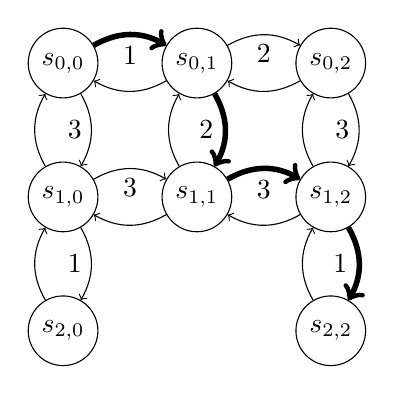
\begin{tikzpicture}
            \tikzset{Vertex/.style={%
                shape=circle,%
                draw=black,%
                minimum size=10pt,%
                radius=1cm,%
                inner sep=3pt,%
                node distance=1.7cm,%
            }}
    
            \node[Vertex] (v00) at (0,0) {$s_{0,0}$};
            \node[Vertex, right of=v00] (v01) {$s_{0,1}$};
            \node[Vertex, right of=v01] (v02) {$s_{0,2}$};
            \node[Vertex, below of=v00] (v10) {$s_{1,0}$};
            \node[Vertex, right of=v10] (v11) {$s_{1,1}$};
            \node[Vertex, right of=v11] (v12) {$s_{1,2}$};
            \node[Vertex, below of=v10] (v20) {$s_{2,0}$};
            \node[Vertex, below of=v12] (v22) {$s_{2,2}$};
    
            \path (v00) edge[->,line width=2pt, bend left] node[below]{1} (v01);
            \path (v01) edge[->, bend left] node[above]{} (v00);

            \path (v01) edge[->, bend left] node[below]{2} (v02);
            \path (v02) edge[->, bend left] node[above]{} (v01);

            \path (v10) edge[->,bend left] node[below]{3} (v11);
            \path (v11) edge[->,bend left] node[above]{} (v10);

            \path (v11) edge[->,bend left,line width=2pt] node[below]{3} (v12);
            \path (v12) edge[->,bend left] node[above]{} (v11);
    
            \path (v00) edge[->,bend left] node[left]{3} (v10);
            \path (v10) edge[->,bend left] node[right]{} (v00);

            \path (v10) edge[->,bend left] node[left]{1} (v20);
            \path (v20) edge[->,bend left] node[right]{} (v10);

            \path (v01) edge[->,bend left,line width=2pt] node[left]{2} (v11);
            \path (v11) edge[->,bend left] node[right]{} (v01);

            \path (v02) edge[->,bend left] node[left]{3} (v12);
            \path (v12) edge[->,bend left] node[right]{} (v02);

            \path (v12) edge[->,bend left,line width=2pt] node[left]{1} (v22);
            \path (v22) edge[->,bend left] node[right]{} (v12);
        \end{tikzpicture}
        $$s_{0,0} \rightarrow s_{0,1} \rightarrow s_{1,1} \rightarrow s_{1,2} \rightarrow s_{2,2}$$
    \end{minipage}%
    \begin{minipage}{0.1\textwidth}
        $\mbox{\Huge $\Rightarrow$}$
    \end{minipage}%
    \begin{minipage}{0.45\textwidth}
        \begin{center}
            \textbf{``Perturbated'' Map}\\
        \end{center}
        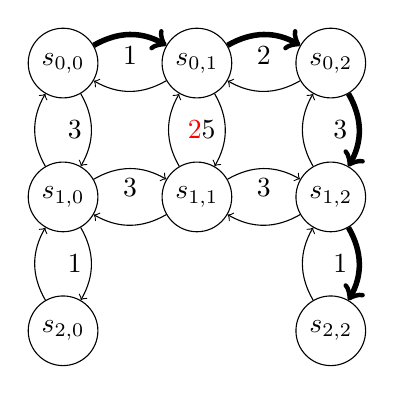
\begin{tikzpicture}
            \tikzset{Vertex/.style={%
                shape=circle,%
                draw=black,%
                minimum size=10pt,%
                radius=1cm,%
                inner sep=3pt,%
                node distance=1.7cm,%
            }}
    
            \node[Vertex] (v00) at (0,0) {$s_{0,0}$};
            \node[Vertex, right of=v00] (v01) {$s_{0,1}$};
            \node[Vertex, right of=v01] (v02) {$s_{0,2}$};
            \node[Vertex, below of=v00] (v10) {$s_{1,0}$};
            \node[Vertex, right of=v10] (v11) {$s_{1,1}$};
            \node[Vertex, right of=v11] (v12) {$s_{1,2}$};
            \node[Vertex, below of=v10] (v20) {$s_{2,0}$};
            \node[Vertex, below of=v12] (v22) {$s_{2,2}$};
    
            \path (v00) edge[->,line width=2pt, bend left] node[below]{1} (v01);
            \path (v01) edge[->, bend left] node[above]{} (v00);

            \path (v01) edge[->,line width=2pt, bend left] node[below]{2} (v02);
            \path (v02) edge[->, bend left] node[above]{} (v01);

            \path (v10) edge[->,bend left] node[below]{3} (v11);
            \path (v11) edge[->,bend left] node[above]{} (v10);

            \path (v11) edge[->,bend left] node[below]{3} (v12);
            \path (v12) edge[->,bend left] node[above]{} (v11);
    
            \path (v00) edge[->,bend left] node[left]{3} (v10);
            \path (v10) edge[->,bend left] node[right]{} (v00);

            \path (v10) edge[->,bend left] node[left]{1} (v20);
            \path (v20) edge[->,bend left] node[right]{} (v10);

            \path (v01) edge[->,bend left] node[left]{{\color{red} \xcancel{2}}{5}} (v11);
            \path (v11) edge[->,bend left] node[right]{} (v01);

            \path (v02) edge[->,bend left,line width=2pt] node[left]{3} (v12);
            \path (v12) edge[->,bend left] node[right]{} (v02);

            \path (v12) edge[->,bend left,line width=2pt] node[left]{1} (v22);
            \path (v22) edge[->,bend left] node[right]{} (v12);
        \end{tikzpicture}
        $$s_{0,0} \rightarrow s_{0,1} \rightarrow s_{0,2} \rightarrow s_{1,2} \rightarrow s_{2,2}$$
    \end{minipage}
\end{frame}

\begin{frame}{Talk Outline}
    \begin{itemize}
        \item Context and Background:
        \begin{itemize}
            \item Compress Path Database (\CPD{});
            \item \ALT{}, \AWA{};
        \end{itemize}
        \item Proposed Techniques: \CPDSearch{} and \anytimeCPDSearch{};
        \item Experimental Results: 
            \begin{itemize}
                \item optimal and 
                \item anytime scenario;
            \end{itemize}
        \item Conclusion and Future Works;
    \end{itemize}
\end{frame}